\chapter{Формулы расчета излучения}\label{Formulae}

\section{Преобразование функции распределения фотонов}
Функция распределения фотонов задана в сферических координатах $n_{ph}(\epsilon,\mu,\phi)$. Рассмотрим переход в систему отсчета, движущуюся в направлении оси $z$ с лоренц-фактором $\gamma = 1/\sqrt{1-\beta^2}$. Количество частиц в элементе фазового пространства $N$ - инвариант.

\begin{equation}
	N = n_{ph}(\epsilon,\mu,\phi)d\epsilon d\mu d\phi dV = n'_{ph}(\epsilon',\mu',\phi')d\epsilon' d\mu' d\phi' dV'
\end{equation}

Для вычисления функции распределения движущейся системе отсчета необходимо вычислить якобиан матрицы перехода в движущуюся систему отсчета. С учеом того, что азимутальный угол $\phi' = \phi$ не изменяется при преобразованиях, и энергия и полярный угол не зависят от объема, занимаемого частицами, в общем виде матрица перехода выглядит как

\begin{equation}\label{generalJacobi}
J=\left(
\begin{array}{cccc}
\frac{d\epsilon'}{d\epsilon} & \frac{d\epsilon'}{d\mu}& 0 & 0\\
\frac{d\mu'}{d\epsilon} & \frac{d\mu'}{d\mu} & 0 & 0\\
0 & 0 & 1 & 0\\
\frac{dV'}{d\epsilon} & \frac{dV'}{d\mu} & 0 & \frac{dV'}{dV}
\end{array}
\right)
\end{equation}

Определитель такой матрицы можно разложить по последнему столбцу и получить, что

\begin{equation}
|J|=\frac{dV'}{dV}\left(\frac{d\epsilon'}{d\epsilon}\frac{d\mu'}{d\mu} - \frac{d\epsilon'}{d\mu}\frac{d\mu'}{d\epsilon}\right)
\end{equation}

Начнем с преобразования пространственного объема $V$. Один способ, используемый в п.10 т.2 Ландау-Лифшица \cite{LandauLifshitz2}, связан с переходом в собственную систему отсчета пучка движущихся частиц. Из этого можно получить, что объем преобразуется обратно энергии $dV'/dV= \epsilon/\epsilon'$. Этот результат правильный, но вывод не корректен для безмассовых частиц, у которых не существует собственной системы отсчета.

Поэтому мы вычислим изменение объема, содержащего рассматриваемые частицы. непосредственно из преобразований Лоренца. Рассмотрим поток частиц, равномерно распределенных вдоль оси $z$, с расстоянием $L$ между соседними частицами, и движущихся со одной скоростью $v$, направленной под углом $\theta$ к оси $z$ и введем величину $\mu = cos \theta$, как показано на рисунке \ref{VolumeTransform}.

\begin{figure}[h]
	\centering
	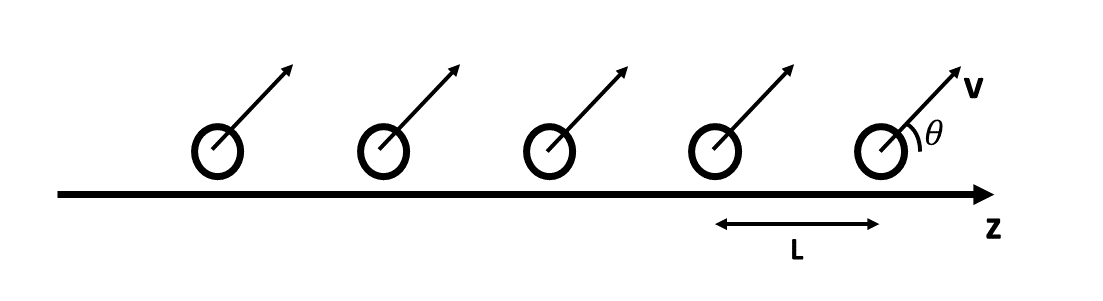
\includegraphics[width=12.5 cm]{./fig/VolumeTransform.png} 
	\caption{Пучок равномерно распределенных частиц, движущихся с одинаковыми скоростями}
	\label{VolumeTransform}
\end{figure}

В лабораторной системе i-тая частица в момент времени t имеет z-координату $z_i = i\cdot L + \mu v t$. Вычислим ее координаты в движущейся системе отсчета

\begin{equation}\label{lorentz_z}
\left(\begin{array}{c}
ct'\\
z'_i
\end{array}
\right)
= \left(
\begin{array}{cc}
\gamma & -\beta\gamma\\
-\beta\gamma & \gamma
\end{array}
\right)
\times
\left(\begin{array}{c}
ct\\
z_i
\end{array}
\right)
\end{equation}  

из этой системы можно получить, что значение координаты в движущейся системе равно $z'_i = \gamma z_i + (\gamma \mu v - c\beta \gamma)t$, но эти значения соответствуют одному моменту времени $t$ в лабораторной системе отсчета, в то время как для определения объема или концентрации в движущейся системе, нам нужны координаты частиц в один момент времени относительно движущейся системы. Поэтому выразим $t$ через $z_i$ и $t'$ и подставим в выражение для координат $z'_i$

\begin{equation}
t=\frac{t'+\gamma\beta z_i/c}{\gamma - \beta \mu v/c}
\end{equation}

и

\begin{equation}
z'_i=\gamma z_i +(\gamma \mu v - c\beta \gamma)\frac{t'+\gamma\beta z_i/c}{\gamma - \beta \mu v/c}=z_i\frac{1}{\gamma(1-\beta\mu v/c)} + t'\frac{\mu v/c - \beta}{1 - \beta \mu v/c}
\end{equation}

Второй член, содержащий $t'$ дает стандартную формулу для релятивистского сложения скоростей. А первый характеризует сокращение расстояний между частицами $L' = z'_{i+1}-z'_i = L/(\gamma(1-\beta\mu v/c))$. Расстояния вдоль поперечных направлений не изменяются, поэтому изменение объема будет таким же

\begin{equation} \label{volume}
V' = V/(\gamma(1-\beta\mu v/c))
\end{equation}

это тот же результат, что и приводимый Ландау и Лифшицем \cite{LandauLifshitz2}

Далее нужно найти выражения для $\epsilon'$ и $\mu'$, но их лучше рассмотреть в двух отдельных случаях - для безмассовых частиц и для массивных.

\subsection{Фотоны}

Рассмотрим преобразование вектора четырех-импульса для безмассовых частиц (фотонов), учитывая что оперечные компоненты не изменяются, а временная и продольная связаны как $p_z = \mu \epsilon$:

\begin{equation}\label{lorentz_ph}
	\left(\begin{array}{c}
		\epsilon'\\
		\mu'\epsilon'
	\end{array}
	\right)
	= \left(
	\begin{array}{cc}
		\gamma & -\beta\gamma\\
		-\beta\gamma & \gamma
	\end{array}
	\right)
	\times
	\left(\begin{array}{c}
		\epsilon\\
		\mu\epsilon
	\end{array}
	\right)
\end{equation}

Из первой строчки матрицы получаем уравнение для допплеровского сдвига энергии

\begin{equation}\label{doppler_ph}
	\epsilon'=\gamma(1-\mu\beta)\epsilon
\end{equation}

Вычислим производные новой энергии по старым координатам

\begin{equation}
	\frac{d\epsilon'}{d\epsilon}=\gamma(1-\mu\beta)
\end{equation}

\begin{equation}
	\frac{d\epsilon'}{d\mu}=-\gamma\beta\epsilon
\end{equation}

Из второй строчки матрицы получаем $\mu'\epsilon'=-\beta\gamma\epsilon+\gamma\mu\epsilon$.Подставив значение $\epsilon'$ из \ref{doppler_ph} и сократив $\epsilon$ получим уравнение аберрации света

\begin{equation}\label{aberration_ph}
	\mu'=\frac{\mu-\beta}{1-\mu\beta}
\end{equation}

Заметим, что угол наклона луча в новой системе не зависит от энергии в старой системе. Вычислим частноую производную $\frac{d\mu'}{d\mu}$

\begin{equation}
	\frac{d\mu'}{d\mu}=\frac{d}{d\mu}\frac{1}{\beta}\frac{\beta\mu-1+1-\beta^2}{1-\mu\beta}=\frac{d}{d\mu}\frac{1}{\beta}\frac{1-\beta^2}{1-\mu\beta}=\frac{1-\beta^2}{(1-\mu\beta)^2}=\frac{1}{\gamma^2(1-\mu\beta)^2}
\end{equation}

Матрица якоби преобразования координат выглядит следующим образом

\begin{equation}
	J=\left(
	\begin{array}{cccc}
		\frac{d\epsilon'}{d\epsilon} & \frac{d\epsilon'}{d\mu}& 0 & 0\\
		0 & \frac{d\mu'}{d\mu} & 0 & 0\\
		0 & 0 & 1 & 0\\
		0 & \frac{dV'}{d\mu} & 0 & \frac{dV'}{dV}
	\end{array}
	\right)
\end{equation}

При такой матрице якобиан, к счастью, равен произведению диагональных членов

\begin{equation}\label{jacobian_ph}
	\frac{D(\epsilon',\mu',\phi',V')}{D(\epsilon,\mu,\phi,V)}=\frac{d\epsilon'}{d\epsilon}\frac{d\mu'}{d\mu}\frac{dV'}{dV}=\gamma(1-\mu\beta)\frac{1}{\gamma^2(1-\mu\beta)^2}\frac{1}{\gamma(1-\mu\beta)}=\frac{1}{\gamma^2(1-\mu\beta)^2}
\end{equation}

И в итоге функция распределения фотонов преобразуется с помощью деления на вычисленный якобиан

\begin{equation}\label{distribution_ph}
	n'_{ph}(\epsilon',\mu',\phi') = \frac{n_{ph}(\epsilon,\mu,\phi)}{\frac{D(\epsilon',\mu',\phi',V')}{D(\epsilon,\mu,\phi,V)}}=\gamma^2(1-\mu\beta)^2 n_{ph}(\epsilon,\mu,\phi)
\end{equation}

\subsection{Массивные частицы}

Для массивных частиц выражения для $\epsilon'$ и $\mu'$ намного сложнее. В этом случае $p_z = \mu \sqrt{\epsilon^2 - m^2 c^4}/c$ где $m$ масса частиц, и преобразования Лоренца выглядят следующим образом

\begin{equation}\label{lorentz_m}
\left(\begin{array}{c}
\epsilon'\\
\mu'\sqrt{{\epsilon'}^2 - m^2 c^4}
\end{array}
\right)
= \left(
\begin{array}{cc}
\gamma & -\beta\gamma\\
-\beta\gamma & \gamma
\end{array}
\right)
\times
\left(\begin{array}{c}
\epsilon\\
\mu\sqrt{{\epsilon}^2-m^2 c^4}
\end{array}
\right)
\end{equation}

и выражения для $\epsilon'$ и $\mu'$

\begin{equation}
\epsilon' = \gamma\epsilon-\beta\gamma\mu\sqrt{\epsilon^2-m^2 c^4}
\end{equation}

\begin{equation}
\mu' = \frac{-\beta\gamma\epsilon+\gamma\mu\sqrt{{\epsilon}^2-m^2 c^4}}{\sqrt{{\epsilon^2 - m^2 c^4}}}
\end{equation}

Выражения для преобразования объемав переменных $\epsilon$ и $\mu$

\begin{equation}
V'=\frac{V}{\gamma(1-\mu\beta\sqrt{{\epsilon}^2-m^2 c^4}/\epsilon)}
\end{equation}

Выражения для частных производных $\epsilon'$, $\mu'$, $V'$ и особенно для якобиана выглядят устрашающе, поэтому здесь мы приведем только финальный результат преобразования функции распределения в единицах $c = 1$

\begin{equation}
\frac{n'_{m}(\epsilon',\mu',\phi')}{n_{m}(\epsilon,\mu,\phi)}= \frac{\gamma(\epsilon-\mu\sqrt{{\epsilon}^2-m^2}\beta)(\gamma^2\epsilon^2-m^2 + \mu^2 ((\epsilon^2-m^2)(\gamma^2-1)) - 2\mu\epsilon\gamma^2\beta\sqrt{\epsilon^2-m^2})^{3/2}}{\epsilon(((\gamma^2-1)(\epsilon^2-m^2)\mu^2 + \gamma^2\epsilon^2 - m^2)\sqrt{\epsilon^2-m^2}-2\mu\epsilon\gamma(\epsilon^2 - m^2)\sqrt{\gamma^2 - 1})}
\end{equation}

\section{Комптоновское рассеяние}\label{ComptonFormulae}
Рассмотрим рассеяние фотонов на одном электроне, движущемся вдоль ось z, см \cite{Dubus}. Сечение Клейна-Нишины в системе покоя электрона равно

\begin{equation}\label{KleinNishina}
\frac{d\sigma}{d\epsilon_1'd\Omega_1'}=\frac{{r_e}^2}{2}\left(\frac{\epsilon_1'}{\epsilon_0'}\right)^2\left(\frac{\epsilon_1'}{\epsilon_0'}+\frac{\epsilon_0'}{\epsilon_1'}-\sin^2\Theta'\right) \delta\left(\epsilon_1' - \frac{\epsilon_0'}{1+\frac{\epsilon_0'}{m_e c^2}(1 - \cos \Theta')}\right)
\end{equation}

Где $r_e$ - классический радиус электрона, $\epsilon_0'$ и $\epsilon_1'$ - энергии начального и конечного фотона, соответственно, $\Theta'$ - угол между начальным и конечным фотоном, определяемый выражением $\cos\Theta' =\cos \theta_0' \cos \theta_1' + \sin \theta_0' \sin \theta_1' \cos(\phi_1' - \phi_0')$. Штрихованные индексы относятся к системе отсчета электрона. При этом начальная и конечная энергии фотонов оказываются связаны соотношениями

\begin{equation}
	\epsilon_1'=\frac{\epsilon_0'}{1+\frac{\epsilon_0'}{m_e c^2}(1 - \cos \Theta')}	
\end{equation}

\begin{equation}
	\epsilon_0'=\frac{\epsilon_1'}{1-\frac{\epsilon_1'}{m_e c^2}(1 - \cos \Theta')}
\end{equation}

Число фотонов, рассеявшихся в заданный телесный угол в единицу времени в промежуток энергии в системе покоя электрона равно

\begin{equation}
\frac{dN'}{dt'd\epsilon_1'd\Omega_1'}=\int c \frac{d\sigma}{d\epsilon_1'd\Omega_1'} \frac{dn'}{d\epsilon_0'd\Omega_0'}d\Omega_0'd\epsilon'_0
\end{equation}

Перепишем дельта-функцию через энергию начального фотона с помощью соотношения 

\begin{equation}
	\delta(f(x)) = \sum \frac{\delta(x-x_k)}{|f'(x_k)|}
\end{equation}

где $x_k$ - корни функции $f(x)$. Производная выражения внутри дельта-функции равна

\begin{equation}
	\frac{d\epsilon_1'}{d\epsilon_0'}=\frac{1}{(1+\frac{\epsilon_0'}{m_e c^2}(1 - \cos \Theta'))^2}
\end{equation}

и она сократится с квадратом отношения энергий в формуле для сечения. Функцию распределения начальных фотонов выразим в лабораторной системе с помощью выражения \ref{distribution_ph}.

\begin{equation}
\frac{dN'}{dt'd\epsilon_1'd\Omega_1'}=\int \frac{r_e^2 c}{2} \gamma_e^2 (1 - \mu_0 \beta_e)^2 \left(\frac{\epsilon_1'}{\epsilon_0'}+\frac{\epsilon_0'}{\epsilon_1'}-\sin^2\Theta'\right)\frac{dn}{d\epsilon_0 d\Omega_0} \delta\left(\epsilon_0' - \frac{\epsilon_1'}{1-\frac{\epsilon_1'}{m_e c^2}(1 - \cos \Theta')}\right) d\epsilon_0'd\mu_0' d\phi_0'
\end{equation}

Теперь избавимся от дельта-функции, проинтегрировав по $\epsilon'_0$.

\begin{equation}
\frac{dN'}{dt'd\epsilon_1'd\Omega_1'}=\int \frac{r_e^2 c}{2} \gamma_e^2 (1 - \mu_0 \beta_e)^2 \left(1 + \cos^2\Theta'+\left(\frac{\epsilon_1'}{m_e c^2}\right)^2\frac{(1-\cos\Theta')^2}{1-\frac{\epsilon_1'}{m_e c^2}(1 - \cos \Theta')}\right)\frac{dn}{d\epsilon_0 d\Omega_0}d\mu_0' d\phi_0'
\end{equation}

Осталось перевести количество рассеяных фотонов в лабораторную систему отсчета $\frac{dN}{dt d\epsilon_1 d\Omega_1} = \frac{dN'}{dt' d\epsilon_1' d\Omega_1'}\frac{dt'}{dt}\frac{d\epsilon_1'}{d\epsilon_1}\frac{d\Omega_1'}{d\Omega_1}$. Используя то, что $dt = \gamma_e dt'$, $\epsilon = \frac{1}{\gamma_e(1 -\mu_1\beta_e)}\epsilon'$ и $\mu_1' = \frac{\mu_1-\beta_e}{1-\mu_1 \beta_e}$ получим

\begin{equation} \label{compton_elframe}
\frac{dN}{dt d\epsilon_1 d\Omega_1}=\int \frac{r_e^2 c}{2} \frac{(1 - \mu_0 \beta_e)^2}{1-\mu_1\beta_e} \left(1 + \cos^2\Theta'+\left(\frac{\epsilon_1'}{m_e c^2}\right)^2\frac{(1-\cos\Theta')^2}{1-\frac{\epsilon_1'}{m_e c^2}(1 - \cos \Theta')}\right)\frac{dn}{d\epsilon_0 d\Omega_0}d\mu_0' d\phi_0'	
\end{equation}

Так же может быть удобно интегрировать в переменных лабораторной системы расчета, тогда выражение для потока фотонов будет следующим

\begin{equation}\label{compton_labframe}
\frac{dN}{dt d\epsilon_1 d\Omega_1}=\int \frac{r_e^2 c}{2} \frac{1}{\gamma_e^2(1-\mu_1\beta_e)} \left(1 + \cos^2\Theta'+\left(\frac{\epsilon_1'}{m_e c^2}\right)^2\frac{(1-\cos\Theta')^2}{1-\frac{\epsilon_1'}{m_e c^2}(1 - \cos \Theta')}\right)\frac{dn}{d\epsilon_0 d\Omega_0}d\mu_0 d\phi_0
\end{equation}

При интегрировании нужно выразить углы в лабораторной системе отсчета $\mu_0, \phi_0$ через переменные интегрирования $\mu_0', \phi_0'$. Для расчета рассеяния на распределении электронов нужно проинтегрировать формулу \ref{compton_elframe} или \ref{compton_labframe} с функцией распределения электронов, нормированной на концентрацию частиц частиц. При этом надо учесть разные направления движения электронов и произвести повороты углов.

В коде реализовано вычисления потоков в терминах энергетической плотности потока энергии в единицах $\textbf{см}^{-2}\textbf{с}^{-1}$. Для вычисления этой величины нужно домножить число рассеянных фотонов на энергию, поделить на квадрат расстояния до источника и проинтегрировать по объему источника.

\begin{equation}\label{comtonKlein}
F(\epsilon_1)=\frac{\epsilon_1}{D^2}\int \frac{dN}{dt d\epsilon_1 d\Omega_1} \frac{dn_e}{d\epsilon_e d\Omega_e} dV d\epsilon_e d\Omega_e
\end{equation}

При рассмотрении процессов, связанных с электронами высоких энергий $\gamma_e \approx 10^8$ относительные численные погрешности вычислений могут быть очень велики, так как $\beta_e$ и $\mu_0, \mu_1, \cos \Theta'$ оказываются слишком близки к единице и стандартный тип double может не разрешать это отличие. Поэтому для численных вычислений оказывается полезным ввести следующие вспомогательные величины:

\begin{equation}
	\delta_e = 1 - \beta_e
\end{equation}

\begin{equation}
	\text{versin}~\theta = 1 - \cos \theta
\end{equation}

Тогда выражения вида $1 - \mu \beta_e$ в этих величинах перепишется как

\begin{equation}
	1 - \mu \beta_e =\text{versin}~\theta + \delta_e - \text{versin}~\theta~\delta_e
\end{equation}

а выражение для угла между конечным и начальным фотоном как

\begin{equation}
	1 - \cos \Theta' = \text{versin}~\theta_0' + \text{versin}~\theta_1' - \text{versin}~ \theta_0' \text{versin}~\theta_1' - \sin \theta_0'\sin \theta_1' \cos(\phi_1'-\phi_0')
\end{equation}

С использованием данных выражений значительно повышается точность и максимальные доступные к рассмотрению энергии фотонов и электронов.

В случае изотропных функций распределения фотонов и релятивистских электронов можно произвести аналитическое интегрирование по угловым переменным \cite{JonesCompton, BykovUvarov2000}, и тогда для вычисления излучения достаточно лишь провести интегрирования по энергиям по формуле

\begin{equation}
F(\epsilon_1)=\frac{\epsilon_1}{D^2}\int \frac{2 \pi r_e^2 \beta_e c}{\epsilon_0 \gamma_e^2} \frac{dn_{ph}}{d\epsilon_0}\frac{dn_e}{d\epsilon_e}(2 q~ \ln(q)+1+q-2q^2+\frac{q^2(1-q)\Gamma^2}{2(1+q\Gamma)})d\epsilon_0 d\epsilon_e dV
\end{equation}

где $\Gamma=4\epsilon_0\gamma_e/m_e c^2$, $q=\epsilon_1/((\gamma_e m_e c^2-\epsilon_1)\Gamma)$.

\section{Синхротронное излучение}\label{SynchrotronFormulae}
Процесс синхротронного излучения хороши известен и описан в классических работах, например \cite{Ginzburg1975}. Но так же возможен и процесс синхротронного поглощения. Сечение этого процесса описано в работе Гизеллини и Свенсона \cite{Ghisellini1991}. В коде вычисляются спектральная плотность мощности излучения единицы объема и линейный коэффициент поглощения, описанные в работе \cite{Ghisellini}. Спектральная плотность мощности излучения единицы объема вещества определеяется формулой

\begin{equation} \label{emission}
	I(\nu)=\int_{E_{min}}^{E_{max}} dE \frac {\sqrt {3}{e}^{3}n F(E) B \sin ( \phi)}{{m_e}{c}^{2}}
	\frac{\nu}{\nu_c}\int_{\frac {\nu}{\nu_c}}^{\infty }\it K_{5/3}(x)dx,
\end{equation}

где $\phi$ это угол межде вектором магнитного поля и лучом зрения, $\displaystyle\nu_{c}$ критическая частота, определяемая выражением $\displaystyle\nu_{c} = 3 e^{2} B \sin(\phi) E^{2}/4\pi {m_{e}}^{3} c^{5}$, и~$K_{5/3}$ - функция МакДональда.
Коэффициент поглощения для фотонов, распростроняющихся вдоль луча зрения равен

\begin{equation}\label{absorption}
	k(\nu)=\int_{E_{min}}^{E_{max}}dE\frac {\sqrt {3}{e}^{3}}{8\pi m_e \nu^2}\frac{n B\sin(\phi)}{E^2}
	\frac{d}{dE} E^2 F(E)\frac {\nu}{ \nu_c}\int_{\frac {\nu}{ \nu_c}}^{\infty }K_{5/3}(x) dx.
\end{equation}

Чтобы вычислить наблюдаемый поток в случае пренебрежимо малого самопоглощения, необходимо проинтегрировать мощность излучения  \ref{emission} по объему источника и поделить результат на квадрат расстояния до источника  $D$. Если самопоглощение значительно, нужно сначала решить дифференциальное уравнение для потока излучения $\Phi=\frac{dW}{dt d\nu dS}$ вдоль луча зрения,

\begin{equation}
	\frac{d\Phi(\nu,z)}{dz} = \frac{dW(\nu)}{dt d\nu dV} - k(\nu)\Phi(\nu,z)
\end{equation}

а затем проинтегрировать по поперечным направлениям

\begin{equation}
	F(\nu)=\frac{1}{D^2}\int dS(x,y) \Phi(\nu, x,y,z_{max})
\end{equation}

где $z_{max}$ - координата поверхности источника.

\subsection*{Синхротронные потери}

В случае изотропного релятивистского распределения электронов, средняя потеря одним электроном описывается как

\begin{equation}
	\frac{dE}{dt} = -\frac{4}{3} \sigma_T c \frac{B^2}{8 \pi} \gamma_e^2
\end{equation}

где $\sigma_T$ Томпсоновское сечение, а $\gamma_e$ Лоренц-фактор электрона. Можно переписать это выражение как

\begin{equation} \label{synchlosses}
	\frac{dE}{dt} = - \frac{4}{9} \frac{e^4 B^2}{m^4 c^7} E^2
\end{equation}

Введем параметр, характеризующий скорость потерь $l = \frac{4}{9} \frac{e^4 B^2}{m^4 c^7}$, тогда в момент времени $t$ энергия частицы с начальной энергией $E_0$ будет равна

\begin{equation}
	E(t) = \frac{E_0}{1 + E_0 l t}
\end{equation}

Теперь вычислим как изменяется функция распределения электронов из-за синхротронных потерь. Если начальная функция распределения равна $F_0(E_0)$, и потери энергии каждой частицы описываются уравнением \ref{synchlosses}, тогда частицы мигрируют к более низким энергиям и с учетом сохранения числа частиц, функция распределения меняется как

\begin{equation}
	F(E,t) = F_0\left(E_0(E,t)\right) dE_0/dE = F_0\left(\frac{E}{1-E l t}\right)\frac{1}{\left(1 - E l t\right)^2}
\end{equation}

Если величина $l$ не постоянна во времени, тогда во всех уравнениях выше нужно заменить множитель $l t$ на интеграл $\int_0^t l(t')dt'$.

\section{Распад пионов}\label{PionFormulae}

В коде реализовано два способа вычисления спектра гамма фотонов, излученных в процессе распада пионов образовавшихся в результате протон-протонного рассеяния. Более простой описан в работе \cite{Kelner}. Количество фотонов излученных в результате одного рассеяния считается пропорциональным полному сечению неупругого протон-протонного рассеяния, которое можно аппроксимировать следующим образом \cite{Kafexhiu}

\begin{equation}\label{sigmainel}
	\sigma_{inel} = \left(30.7 - 0.96\ln\left(E_p/E_{th}\right) + 0.18\ln^2\left(E_p/E_{th}\right) \right)\times\left(1 - \left(E_{th}/E_p\right)^{1.9}\right)^3\cdot10^{-27} \text{см}^{2}
\end{equation}

где $E_p$ кинетическая энергия ускоренного протона, $E_{th}$ пороговая энергия реакции $E_{th} = 2m_{\pi}+m^2_{\pi}/2m_p \approx 0.2797~\text{GeV}$

Количество фотонов излученных в единицу энергии $\left(\epsilon, \epsilon+d\epsilon\right)$ в единицу объема в единицу времени равно

\begin{equation}
	\frac{dN}{dt d\epsilon dV} = c n_{amb} \int_{\epsilon}^{\inf}\sigma_{inel}(E_p)F(E_p)F_{\gamma}(\epsilon/E_p, E_p) dE_p/E_p
\end{equation} 

где $n_{amb}$ концентрация фоновых протонов, а функция $F_{\gamma}(\epsilon/E_p, E_p)$ определена как

\begin{equation}
	F_{\gamma}(x, E_p) = B \frac{\ln(x)}{x} \left(\frac{1-x^\beta}{1+k x^{\beta}\left(1-x^\beta\right)}\right)^4\times\left(\frac{1}{\ln(x)}-\frac{4\beta x^\beta}{1-x^\beta}-\frac{4 k\beta x^\beta\left(1-2x^\beta\right)}{1+k x^\beta\left(1-x^\beta\right)}\right)
\end{equation}

Параметры $B, \beta, k$ зависят только от энергии ускоренного протона и в диапазоне энергий $0.1~\text{ТэВ} < E_p < 10^5~\text{ТэВ}$ могут быть выражены как $B = 1.3 + 0.14 L + 0.011 L^2$, $\beta = 1.0/\left(1.79 + 0.11 L  + 0.008 L^2\right)$ и $k = 1.0/\left(0.801 + 0.049 L + 0.014 L^2\right)$, где $L = \ln\left(E_p/1~\text{ТэВ}\right)$

В более сложной модели, описанной в работе \cite{Kafexhiu}, на низких энергиях ($E_p < 2~\text{ГэВ}$) используется непосредственно сечение рождение пионов, в то время как на высоких используется доля полного сечения неупругого рассеяния $\sigma_{inel}$, но с более точными поправочными коэффициентами.

На низких энергиях сечение рождения пионов  $\sigma_{\pi}$ складывается из сечений трех процессов - с рождением одного пиона $pp\rightarrow pp\pi^0$ и с рождением двух пионов $pp\rightarrow pp2\pi^0$ и $pp\rightarrow \{pn,D\}\pi^{+}\pi^0$. Первое сечение выражается как

\begin{equation}
	\sigma_{1\pi} = 7.66\times10^{-30}\eta^{1.95}\left(1 + \eta + \eta^5\right)\times\left(f_{BW}\left(\sqrt s\right)\right)^{1.86}~\text{см}^{2}
\end{equation}

где $s = 2 m_p \left(E_p+2m_p\right)$ квадрат энергии в системе центра инерции, $\eta$ нормированный максимальный импульс пиона

\begin{equation}
	\eta = \frac{\sqrt{\left(s-m_{\pi}^2-4m_p^2\right)^2-16 m_{\pi}^2m_p^2}}{2m_{\pi}\sqrt{s}}
\end{equation}

и $f_{BW}$ релятивистское распределение Брейта-Вигнера

\begin{equation}
	f_{BW}\left(\sqrt{s}\right)=\frac{m_p K}{\left(\left(\sqrt{s}-m_p\right)^2-M_{res}^2\right)^2+M_{res}^2\Gamma_{res}^2}
\end{equation}

где $K = \sqrt{8}M_{res}\Gamma_{res}\gamma/\pi\sqrt{M_{res}^2+\gamma}$ и $\gamma = \sqrt{M_{res}^2\left(M_{res}^2+\Gamma_{res}^2\right)}$. Значения используемых параметров равны $M_{res} = 1.1883~\text{ГэВ}$ и $\Gamma_{res} = 0.2264~\text{ГэВ}$.

Полное сечение процессов, в которых рождаются два пиона, равно

\begin{equation}
	\sigma_{2\pi}=\frac{5.7\cdot10^{-27}}{1+\exp(-9.3\left(E_p/1~\text{GeV} - 1.4\right))}
\end{equation}

Для энергий $E_p > 0.56~\text{GeV}$, а для более низких энергий оно равно нулю.

Для энергий выше 2 ГэВ, сечение рождения пиона вычисляется через среднее число рождения пионов при одном столконовении и полное сечение неупругого рассеяния \ref{sigmainel} $\sigma_{\pi} = \braket{n_{\pi}} \sigma_{inel}$. Для энергий меньше 5 ГэВ среднее число рожденных пионов равно $\braket{n_{\pi}} = -0.006 + 0.237 Q - 0.023 Q^2$ где $Q = \left(E_p - E_{th}\right)/m_p$. Для энергий выше 5 ГэВ is $\braket{n_{\pi}} = a_1 \xi^{a_4}\left(1 + \exp\left(-a_2\xi^{a_5}\right)\right)\left(1-\exp\left(-a_3\xi^{1/4}\right)\right)$, где $\xi = \left(E_p/1~\text{ГэВ} - 3\right)/m_p$ и коэффициенты $a_1-a_5$ вычислены с численным моделированием с помощью кода GEANT \cite{AllisonGeant2006}, $a_1 = 0.728, a_2 = 0.596, a_3 = 0.491, a_4 = 0.2503, a_5 = 0.117$.

Теперь, зная $\sigma_{\pi}$, можно выразить сечение излучения фотона в единицу энергии

\begin{equation}
	\frac{d\sigma_{\gamma}\left(E_p, \epsilon\right)}{d\epsilon} = A_{max}\left(E_p\right)\times F\left(E_p, \epsilon\right)
\end{equation}

где $A_{max}(E_p)$ максимум сечения по всем энергиям фотона, который зависит только от энергии протона, а $F\left(E_p,\epsilon\right)$ описывает форму спектра. Для явного выражения $F\left(E_p, \epsilon\right)$ нужно сначала ввести несколько величин, описывающих кинематику. $Y=\epsilon+\frac{m_{\pi}^2}{4 \epsilon}$, $Y_{max}=\epsilon_{max}+\frac{m_{\pi}^2}{4 \epsilon_{max}}$, где $\epsilon_{max}$ максимальная энергия излученного фотона при данной энергии протона, $X=\frac{Y-m_{\pi}}{Y_{max}-m_{\pi}}$. Энергия пиона в системе центра инерции равна $E_{CM}=\frac{s-4m_p^2+m_{\pi}^2}{s\sqrt{s}}$, а максимальная энергия пиона в лабораторной системе -  $E_{max}=\gamma_{CM}\left(E_{CM}+\sqrt{E_{CM}-m_{\pi}^2}\beta_{CM}\right)$, где лоренц-фактор центра инерции в лабораторной системе $\gamma_{CM}=\frac{E_p+2m_p}{\sqrt{s}}$ и $\beta_{CM}=\sqrt{1-1/\gamma_{CM}^2}$. Теперь выражение для $F\left(E_p,\epsilon\right)$ можно записать как
\begin{equation}
	F\left(E_p,\epsilon\right) = \frac{\left(1-X^{\alpha(E_p)}\right)^{\beta(E_p)}}{\left(1+X Y_{max}/\lambda m_{\pi}\right)^{\gamma(E_p)}}
\end{equation}

Янвые выражения для $\lambda, \alpha(E_p), \beta(E_p), \gamma(E_p)$ можно найти в работе \cite{Kafexhiu}.

Величина $A_{max}$ может быть выражена как $5.9\times\frac{\sigma_{\pi}}{E_{max}}$ для протонов с кинетическими энергиями меньше < 1 ГэВ, и как $b_1 \left(E_p/m_p\right)^{-b_2}\exp\left(b_3 \ln^2\left(E_p/m_p\right)\right)\times\frac{\sigma_{\pi}}{m_p}$ для высоких энергий. Выражения для $b_1, b_2, b_3$ так же можно найти в работе \cite{Kafexhiu}. Полное число излученных фотонов в единице времени в единице объема в единицу энергии в интервале энергий $\left(\epsilon, \epsilon + d\epsilon\right)$ может быть найдено интегрированием $\frac{d\sigma_{\gamma}\left(E_p, \epsilon\right)}{d\epsilon}$ с функцией распределения протонов.

\begin{equation}
	\frac{dN}{dt d\epsilon dV} = c n_{amb} \int_{\epsilon}^{\inf}\frac{d\sigma_{\gamma}\left(E_p, \epsilon\right)}{d\epsilon} F(E_p) dE_p
\end{equation} 

\section{Тормозное излучение}\label{BremsstrahlungFormulae}

Для простого случая тормозного излучения горячей плазмы мы используем формулы, описанные в книге \cite{Rybicki}.
Количество энергии, излучаемой в единицу энергии, в единицу времени единицей объема равно

\begin{equation}
	\frac{dW}{dt d\epsilon dV} = \frac{2^5 \pi e^6}{3 h m c^3}\sqrt{\frac{2\pi}{3 k m}}T^{-1/2}Z^2n_e n_i\exp\left(-\frac{\epsilon}{kT}\right)\bar{G}
\end{equation}

где $T$ температура плазмы, $n_e, n_i$ концентрации электронов и ионов соответственно, $Z$ зарядовое число ионов и $\bar{G}$ гаунт-фактор, усредненный по скоростям частиц. Приближенные выражения для $\bar{G}$ приведены в книге Новикова и Торна \cite{NovikovThorne} и исправлены Райбеки и Лайтманом \cite{Rybicki}. Формулы для разных режимов рассеяния - малоуглового и рассеяния на большие углы, а так же для классического и квантового режима, когда становится важен принцип неопределенности (П.Н.), приведены на рисунке \ref{gaunt}, где $R_y$ - постоянная Ридберга и $\xi$ постоянная Эйлера-Маскерони.

\begin{figure}
	\centering
	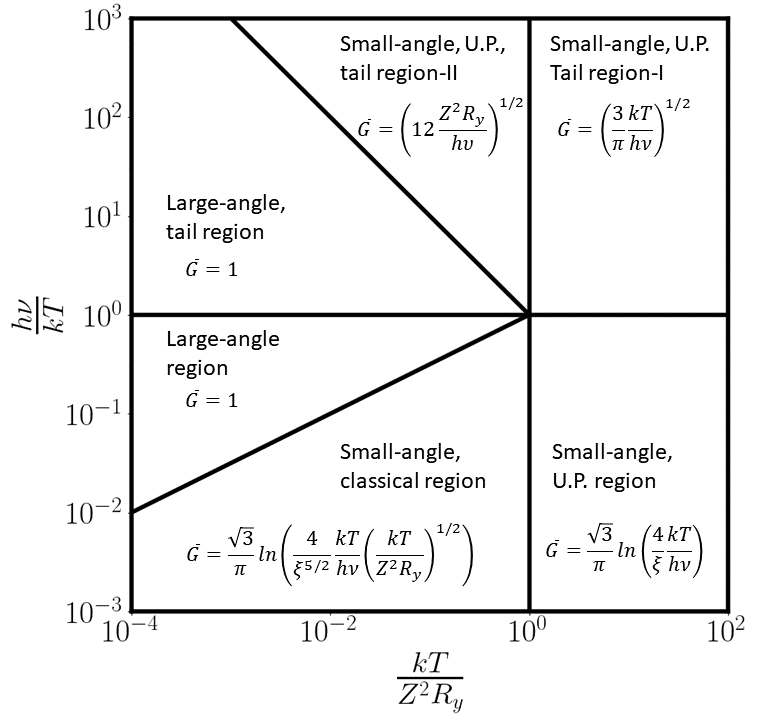
\includegraphics[width=11.5 cm]{./fig/gaunt.png} 
	\caption{Усредненные гаунт-факторы, цитируется по Райбеки и Лайтман \cite{Rybicki}, выведены Новиковым и Торном \cite{NovikovThorne}}
	\label{gaunt}
\end{figure}

Для случая произвольных изотропных распределений рассеивающихся лектронов мы используем уравнения приведенные в работе \cite{Baring1999}. Количество фотонов, излученных в единицу времени в единицу энергии единицей объема заданным распределением электронов определяется как

\begin{equation}
	\frac{dN}{dt d\epsilon dV} = \int\frac{dN_{\gamma}\left(E_e, \epsilon\right)}{dt d\epsilon} F(E_e) dE_e
\end{equation}

где $\frac{dN_{\gamma}\left(E_e, \epsilon\right)}{dt d\epsilon}$ число фотонов излученных одним лектроном с энергией $E_e$. Эту величину можно выразить как

\begin{equation}
	\frac{dN_{\gamma}\left(E_e, \epsilon\right)}{dt d\epsilon} = v_e \left(\left(\sum n_i Z_i^2\right)\sigma_{e-p} + n_e\sigma_{e-e}\right)
\end{equation}

где $v_e$ скорость электрона, $n_i, Z_i$ концентрации и зарядовые числа каждого типа ионов, а $\sigma_{e-p}$ и $\sigma_{e-e}$ сечения электрон-протонного и электрон-электронного рассеяния соответственно.

Электрон-электронное сечение в релятивистском режиме ($E_e > 2~\text{МэВ}$) может быть выражено следующим образом, как показано в работе \cite{BaierJETP1967}

\begin{equation}
\sigma_{e-e}(E_e,\epsilon) = \left(\sigma_1 + \sigma_2\right)A\left(\epsilon, E_e/m_e c^2\right)
\end{equation}

Первый член в скобках определяется как

\begin{equation}\label{sigma1}
	\sigma_1 = \frac{4 r_e^2 \alpha}{\epsilon}\left(1+\left(\frac{1}{3}-\frac{\epsilon}{\gamma_e}\right)\left(1-\frac{\epsilon}{\gamma_e}\right)\right)\left(\ln\left(2\gamma_e\frac{\gamma_e - \epsilon}{\epsilon}\right)-\frac{1}{2}\right)
\end{equation}

Выражение для $\sigma_2$ более сложное и разделяется на два случая. Для $\epsilon < 1/2$:

\begin{equation}
	\begin{split}
		\sigma_2 = \frac{r_e^2\alpha}{3\epsilon} \left( 16 \left( 1-\epsilon+\epsilon^2 \right) \ln\frac{\gamma_e}{\epsilon}-\frac{1}{\epsilon^2}+\frac{3}{\epsilon}-4+4\epsilon-8\epsilon^2 \right. \\ \left. - 2\left( 1-2\epsilon \right) \ln \left( 1-2\epsilon \right) \left( \frac{1}{4\epsilon^3}-\frac{1}{2\epsilon^2}+\frac{3}{\epsilon}-2+4\epsilon \right) \right)
	\end{split}
\end{equation}

и для $\epsilon > 1/2$:

\begin{equation}
	\sigma_2 = \frac{r_e^2\alpha}{3\epsilon}\frac{2}{\epsilon}\left(\left(4-\frac{1}{\epsilon}+\frac{1}{4\epsilon^2}\right)\ln\left(2\gamma_e\right)-2+\frac{2}{\epsilon}-\frac{5}{8\epsilon^2}\right)
\end{equation}

где $r_e$ классический радиус электрона и $\alpha$ постоянная тонкой структуры. Поправочный фактор $A(\epsilon, \gamma_e)$ определяется как

\begin{equation}
	A\left(\epsilon, \gamma_e\right)=1-\frac{8}{3}\frac{\left(\gamma_e-1\right)^5}{\gamma_e + 1}\left(\frac{\epsilon}{\gamma_e}\right)^{1/3}
\end{equation}

В нерелятивистском режиме электрон-электронное сечение равно

\begin{equation}
	\sigma_{NR}=\frac{4r_e^2\alpha}{15\epsilon}F\left(\frac{4\epsilon}{\gamma_e^2-1}\right)
\end{equation}

где

\begin{equation}
	\begin{split}
		F(x) = \left(1+\frac{1}{2}\left(\gamma_e^2-1\right)\right)\left(17-\frac{3x^2}{\left(2-x\right)^2}-\frac{10x\gamma_e\beta_e\left(2+\gamma_e\beta_e\right)}{1+x^2\left(\gamma_e^2-1\right)}\right)\sqrt{1-x} \\ +\left(12\left(2-x\right)-\frac{7x^2}{2-x}-\frac{3x^4}{\left(2-x\right)^3}\right)\ln\frac{1+\sqrt{1-x}}{\sqrt{x}}
	\end{split}
\end{equation}

Сечение для электрон-протонного рассеяния приведено Бёте и Хайтлером в работе \cite{BetheHeitler}. Можно заметить, что в ультрарелятивистском режиме оно равно слагаемому $\sigma_1$ в формуле для электрон-электронного рассеяния \ref{sigma1} \cite{JauchRohrlich}. В общем случае сечение Бёте-Хайтлера равно

\begin{equation}
	\begin{split}
		\sigma_{e-p} = \frac{r_e^2\alpha}{\epsilon}\frac{p'}{p}\left(\frac{4}{3}-\frac{2}{\left(\beta_e\beta_e'\right)^2}\left(\frac{\gamma_e}{\gamma_e'}+\frac{\gamma_e'}{\gamma_e}-\frac{2}{\gamma_e\gamma_e'}\right) + \right. \\ \left. \left(l\frac{\gamma_e'}{\gamma_e^2-1}+l'\frac{\gamma_e}{\gamma_e'^2-1}-l l'\right) + L\left(\frac{8}{3}\gamma_e\gamma_e'+\epsilon^2\left(\frac{1}{\left(\beta_e\beta_e'\right)^2+1}\right)+ \right. \right. \\ \left. \left. \frac{1}{2}\epsilon\left(l\left(1+\frac{\gamma_e'}{\beta_e^2\gamma_e}\right)-l'\left(1+\frac{\gamma_e}{\beta_e'^2\gamma_e'}\right)+2\frac{\epsilon}{\beta_e^2\gamma_e\beta_e'^2\gamma_e'}\right)\right)\right)
	\end{split}
\end{equation}

В этой формуле используются следующие вспомогательные величины: $\gamma_e$ - лоренц-фактор начального электрона, $\beta_e$ - его скорость в единицах скорости света, $l = \frac{1}{\beta_e\gamma_e}\ln\frac{1+\beta_e}{1-\beta_e}$, штрихованные величины относятся к рассеянному электрону и они связаны соотношением $\gamma_e = \gamma_e' + \epsilon$. Так же введена дополнительная величина $L = \frac{2}{\beta_e\gamma_e\beta_e'\gamma_e'}\ln\frac{\gamma_e\gamma_e'\left(1+\beta_e\beta_e'\right)-1}{\epsilon}$.